\section{The Credit Carousel: How Fintech Round-Tripping Keeps Everyone in the Dark}

\vfill

\begin{figure}[H]
  \centering

  % === First row ===
  \begin{subfigure}[t]{0.45\textwidth}
    \centering
    \begin{tikzpicture}
      \comicpanel{0}{0}
        {NeuralScore AI}
        {LendFast Executive}
        {Our models turn risk into revenue.}
        {(0,-0.6)}
    \end{tikzpicture}
    \caption*{The pitch: data as gold, risk as an algorithm.}
  \end{subfigure}
  \hfill
  \begin{subfigure}[t]{0.45\textwidth}
    \centering
    \begin{tikzpicture}
      \comicpanel{0}{0}
        {LendFast Executive}
        {NeuralScore AI}
        {And your fee?}
        {(0,-0.6)}
    \end{tikzpicture}
    \caption*{The price: a cut of every high-risk dollar.}
  \end{subfigure}

  \vspace{1em}

  % === Second row ===
  \begin{subfigure}[t]{0.45\textwidth}
    \centering
    \begin{tikzpicture}
      \comicpanel{0}{0}
        {NeuralScore AI}
        {LendFast Executive}
        {Half a percent per account—and you advertise on our site.}
        {(0,-0.6)}
    \end{tikzpicture}
    \caption*{The arrangement: services for ads, ads for services.}
  \end{subfigure}
  \hfill
  \begin{subfigure}[t]{0.45\textwidth}
    \centering
    \begin{tikzpicture}
      \comicpanel{0}{0}
        {LendFast Executive}
        {NeuralScore AI}
        {Deal. Let’s call it synergy.}
        {(0,-0.6)}
    \end{tikzpicture}
    \caption*{The handshake: where risk meets revenue.}
  \end{subfigure}

  \caption*{In this carousel, the only constant is the circle of capital feeding itself.}
\end{figure}

\subsection{Hypothetical Case Study: NeuralScore AI and LendFast Loans — Predation by Algorithm and Accounting}

\medskip

\begin{HistoricalSidebar}{From Check-Cashers to Clever \emph{Tech}: A Brief History of Predatory Credit}

Predatory lending isn’t new. In the 1990s, \emph{payday lenders} offered short-term loans at triple-digit APRs under the guise of “emergency assistance.” Borrowers trapped in rolling debt cycles couldn’t escape escalating fees. By 2005, some states capped APRs, but lenders simply rebranded, opened new subsidiaries, or moved operations online.

\medskip

Fast-forward to the 2010s: fintech startups claimed to democratize credit through \emph{data-driven underwriting}. In reality, sophisticated models masqueraded as fair algorithms while perpetuating subprime rates—sometimes exceeding 200\% APR—under the cover of “market-based pricing.” Creative accounting and off-balance-sheet vehicles masked toxic debt from regulators and investors alike.

\medskip

The lesson: whether it’s a storefront in a strip mall or an API in the cloud, the same dynamic persists: the lender profits when the borrower can’t pay.

\end{HistoricalSidebar}

\medskip

\textbf{NeuralScore AI} began as a San Francisco startup promising a “transformative credit-scoring engine.” Founded by ex-academics in machine learning, its flagship product—\emph{NeuraScore 2.0}—claimed to predict default probabilities with 97\% accuracy. In reality, the model was intentionally overfitted, calibrated to approve borderline subprime applicants so long as it generated ongoing fee revenue from renewals and late payments.

\medskip

\textbf{LendFast Loans} was a direct-to-consumer lender specializing in subprime credit cards and personal loans. Their rates hovered between 79\% and 259\% APR—legally compliant but economically punishing. LendFast’s branding emphasized “financial inclusion,” complete with stock photos of smiling families. Behind the scenes, they relied almost entirely on NeuralScore’s black-box models to assemble borrower portfolios that maximized fee income.

\medskip

\begin{itemize}
  \item  \textbf{NeuralScore AI charges LendFast} an origination and servicing fee equal to 0.5\% of each loan balance—upfront, capitalized into the debt so the borrower never sees it.
  \item  \textbf{LendFast advertises with NeuralScore}, purchasing \$200{,}000 worth of “promotional credits” on NeuraScore’s dashboard (billed as “data partnership”), which NeuralScore recognizes immediately as revenue.
  \item  \textbf{Round-tripping scam}:
    \begin{enumerate}
      \item  LendFast pays NeuralScore \$2 million in service fees over twelve months.
      \item  NeuralScore books \$2 million in subscription and ad revenue.
      \item  LendFast takes a \$2 million marketing expense deduction; NeuralScore shows top-line growth to investors.
      \item  Meanwhile, LendFast’s loan loss provisions swell under the guise of “variable reserves,” booked off-balance-sheet through a shell entity, \emph{ReserveCo LLC}.
    \end{enumerate}
  \item  \textbf{Creative Accounting}:  ReserveCo holds non-performing loans but sells “portfolios” back to LendFast at inflated values, generating unrealized gains for LendFast’s P\&L—while concealing the true default rates from auditors.
\end{itemize}

By structuring the relationship this way, NeuralScore’s cap table looks pristine: exponential recurring revenue, predictable churn, and no visible loan defaults. LendFast’s income statement similarly appears healthy: “net interest margin” of 40 percentage points, “marketing expense” that aligns with growth, and “data services” booked as a cost—but also as a boon to valuation for NeuralScore. Everyone wins… for a while.

% ------ make sure we are in outer paragraph mode here ------
\begin{figure}[H]
    \centering
    \begin{dot2tex}[dot,options=-t tikz,options=-s -Gnodesep=0.6]
      digraph LendFastDiagram {
        rankdir=LR;
        node [shape=rectangle, style=rounded, fontsize=10];
        
        subgraph cluster_market {
          label="Market";
          style=dashed;
          color=gray;
          Borrowers [label="Borrowers\n(79\%–259\% APR)"];
        }
        
        subgraph cluster_core {
          label="Core Operations";
          style=dashed;
          color=gray;
          LendFast [label="LendFast Loans\n(Subprime Lender)"];
          ReserveCo [label="ReserveCo LLC\n(Off-Balance Reserves)"];
        }
        
        subgraph cluster_model {
          label="Modeling Partner";
          style=dashed;
          color=gray;
          NeuralScore [label="NeuralScore AI\n(Credit Models)"];
        }
        
        Borrowers -> LendFast [label="Loan Repayments\n\& Interest"];
        LendFast -> ReserveCo   [label="Aggregate Reserve\nTransfers"];
        ReserveCo -> LendFast   [label="Portfolios at\nInflated Value"];
        
        LendFast -> NeuralScore [label="0.5\% Origination\n\& Servicing Fees"];
        LendFast -> NeuralScore [label="\$200{,}000 Promo Credits",
                                 style=dotted, arrowhead=vee, constraint=false];
        
        LendFast -> InvLF       [label="Reported Profitable\nMetrics", ltail=cluster_core, lhead=cluster_core];
        NeuralScore -> InvNS    [label="Recognized Revenue", ltail=cluster_model, lhead=cluster_model];
        
        subgraph cluster_roundtrip {
          label="Round-Tripping Scam";
          color=red;
          style=dashed;
          LendFast;
          ReserveCo;
          NeuralScore;
        }
      }
    \end{dot2tex}
    \caption{Flow of funds and “round‐tripping scam” between LendFast Loans, ReserveCo, and NeuralScore AI.}
  \end{figure}
  


\medskip

\begin{PsychologySidebar}{The Allure of “AI Ethics”: When Trust Bias Becomes Exploitable}

Tech executives know that \emph{“AI”} enjoys a halo effect. If an underwriting decision is labeled “AI-driven,” consumers assume objectivity and fairness. Regulators, investors, and even journalists often defer—“Let’s see the code,” they say, but rarely do until it’s too late.

\medskip

Psychologists call this \textbf{automation bias}: the tendency to trust automated decisions over human judgment—even when the former is flawed. NeuralScore exploited this bias by incorporating irrelevant social signals (e.g., measuring “social media engagement” as a proxy for “responsibility”) so their models approved more applicants while still maintaining the veneer of rigorous “big data” science.

\medskip

Meanwhile, LendFast sold the narrative of “inclusion,” invoking empathy for the underbanked. Borrowers internalized a \textbf{just-world belief}: “If the algorithm approves me, I must be creditworthy.” Their denial—“I can handle 200\% APR; it’s a short-term fix”—masked the reality that they were entering a debt spiral engineered to extract maximum fees.

\begin{quote}
The most dangerous bias is the one that feels like empowerment.
\end{quote}

\end{PsychologySidebar}

\medskip

At first glance, the partnership seemed mutually beneficial:

\begin{itemize}
  \item  \textbf{NeuralScore} touted “monetization of data” to its VC backers, demonstrating 50 percent year-over-year growth in revenue from “strategic partners.”
  \item  \textbf{LendFast} signed term sheets with investors at 15\% preferred, using “AI-driven underwriting” as the headline—even though their loss ratio (loans in default) climbed from 8 percent in Q1 to 23 percent by Q4.
  \item  \textbf{ReserveCo LLC} quietly bought non-performing loans at book value from LendFast, then sold them back to a shell called “LF Special Servicing” at marked-up valuations, generating phantom profits later reversed when regulators (belatedly) required higher reserves.
\end{itemize}

All of this remained opaque until one of the external auditors—tasked with reviewing LendFast’s year‐end financials—noticed subtle inconsistencies in the aggregated loan‐loss reserve figures. On the surface, LendFast’s consolidated reserves appeared to follow a smooth, upward trajectory roughly proportional to its reported charge‐off rate. However, when the auditor drilled down into quarterly roll‐forward schedules (which had been presented as a single line item labeled “aggregate reserve adjustment”), he observed that:

\begin{itemize}[nosep]
    \item \textbf{Reserve Ratios Remained Suspiciously Constant}
    \begin{itemize}[nosep]
        \item Across multiple quarters, the overall loan‐loss reserve balance increased by almost exactly the prior quarter’s net charge‐offs, as if LendFast had simply replenished reserves dollar for dollar rather than applying an actuarially determined reserve model.
        \item In a normally functioning portfolio, the reserve‐to‐outstanding‐loans ratio fluctuates with changes in delinquency trends, vintage performance, or economic conditions. Here, though, the ratio hovered at exactly 4.2 \% each quarter—even when delinquencies jumped or reserves should have been materially higher.
    \end{itemize}

    \item \textbf{Hidden Segment Shifts}
    \begin{itemize}[nosep]
        \item LendFast grouped all subprime personal loans, credit card portfolios, and so‐called “variable‐reserve funding facilities” under a single “Consumer Lending” bucket. Within that aggregated total, small but systematic “reclassifications” appeared each quarter—large write‐downs shifted from “unsecured personal loans” to “off‐balance‐sheet reserve vehicles” without adequate explanation.
        \item The auditor traced these shifts in the footnotes: a \$15 million write‐off in Q2 labeled as “loss on sale of loan portfolio” was quietly reclassified one line down as “reserve adjustment for off‐balance‐sheet entity.” That reclassification effectively hid the fact that the actual credit loss was far higher than the aggregate number implied.
    \end{itemize}

    \item \textbf{Unusual Round‐Tripping Adjustments}
    \begin{itemize}[nosep]
        \item Every time the company took on a new tranche of “variable reserves” via ReserveCo LLC, the consolidated reserve amount jumped exactly by the same amount as a corresponding “marketing expense” or “data‐services fee” billed to NeuralScore AI. This pattern showed up consistently, quarter after quarter, with no normal audit‐trail justification.
        \item In essence, LendFast’s net income stayed artificially inflated because the reserves were being replenished by what should have been recorded as operating expenses—hidden inside a broad “service fees” line. Only by isolating ReserveCo‐related entries did the auditor see that \$20 million of what appeared to be legitimate revenue was, in reality, being funneled right back into reserves to mask deteriorating loan performance.
    \end{itemize}
\end{itemize}

Because these irregularities were buried within high‐level aggregates—rather than presented as discrete line items—the initial review procedures didn’t flag them. But when the auditor performed variance analysis on individual loan segments, comparing actual charge‐off trends to the implied reserve build, he realized the “smooth” aggregate numbers couldn’t reconcile with the underlying portfolio performance. That discrepancy ultimately triggered a full forensic review, peeling back several quarters of “magical P/E booster” adjustments and exposing the illusion of profitability and growth.

\begin{figure}[H]
    \centering
  
    % ==== Panel 1: Constant Reserve Ratio ====
    \begin{minipage}{0.9\textwidth}
      \centering
      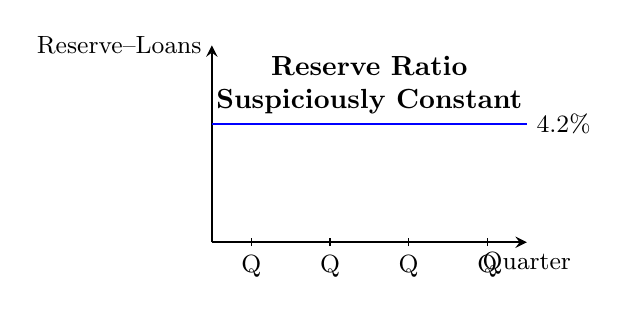
\begin{tikzpicture}[
        font=\small,
        axis/.style={thick, ->, >=stealth},
        label/.style={font=\bfseries, align=center}
      ]
        \node[label] (title1) at (0,1.5) {Reserve Ratio\\Suspiciously Constant};
  
        % Axes
        \draw[axis] (-2,-0.5) -- (-2,2) node[left] {Reserve–Loans};
        \draw[axis] (-2,-0.5) -- (2,-0.5) node[below] {Quarter};
  
        % Flat line at 4.2%
        \draw[thick, blue] (-2,1) -- (2,1);
        \node[right] at (2,1) {4.2\%};
  
        % Quarterly ticks
        \foreach \x in {-1.5,-0.5,0.5,1.5} {
          \draw (\x,-0.55) -- (\x,-0.45);
          \node[below] at (\x,-0.55) {Q};
        }
      \end{tikzpicture}
    \end{minipage}
  
    \vspace{1em}
  
    % ==== Panel 2: Hidden Segment Shifts ====
    \begin{minipage}{0.9\textwidth}
      \centering
      \begin{tikzpicture}[
        font=\small,
        label/.style={font=\bfseries, align=center}
      ]
        \node[label] (title2) at (0,1.5) {Hidden Segment\\Reclassifications};
  
        % Bars for Q2
        \draw[draw=none, fill=gray!30] (-1, -0.5) rectangle ++(0.8,2) node[midway] {Unsecured Loans};
        \draw[draw=none, fill=gray!60] (-1, 1.5) rectangle ++(0.8,1.5) node[midway] {Other Portfolios};
  
        % Bars for Q3
        \draw[draw=none, fill=gray!30] (1, -0.5) rectangle ++(0.8,1.5) node[midway] {Unsecured Loans};
        \draw[draw=none, fill=gray!60] (1, 1.0) rectangle ++(0.8,2) node[midway] {Off-B/S Reserves};
  
        % Reclassification arrow
        \draw[->, red, thick] (-0.2,0.5) to[bend left] (0.8,1.0);
        \node[red, above] at (0.3,0.8) {Reclassify \$15M};
  
        % Quarter labels
        \node[below] at (-0.6,-0.5) {Q2};
        \node[below] at (1.4,-0.5) {Q3};
  
        % Legend
        \node[draw, fill=gray!30, minimum width=0.8cm] (-legA) at (0,-2) {};
        \node[right=3pt of -legA] {“Unsecured Loans”};
        \node[draw, fill=gray!60, minimum width=0.8cm] (-legB) at (0,-2.7) {};
        \node[right=3pt of -legB] {“Off-B/S Reserves”};
      \end{tikzpicture}
    \end{minipage}
  
    \vspace{1em}
  
    % ==== Panel 3: Round‐Tripping Adjustments ====
    \begin{minipage}{0.9\textwidth}
      \centering
      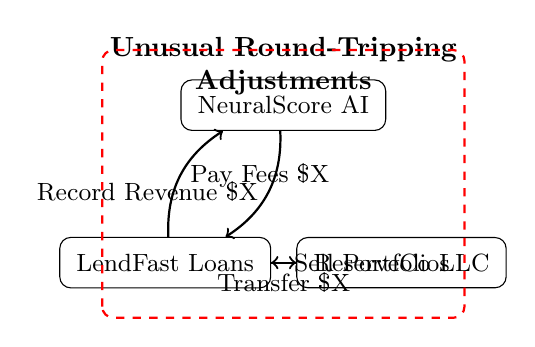
\begin{tikzpicture}[
        font=\small,
        label/.style={font=\bfseries, align=center},
        box/.style={draw, rounded corners, inner sep=6pt, align=center}
      ]
        \node[label] (title3) at (0,1.5) {Unusual Round‐Tripping\\Adjustments};
  
        % Boxes
        \node[box] (LF) at (-1.5,-1) {LendFast Loans};
        \node[box] (RC) at (1.5,-1) {ReserveCo LLC};
        \node[box] (NS) at (0,1) {NeuralScore AI};
  
        % Arrows between them
        \draw[->, thick] (LF) -- node[below] {Transfer \$X} (RC);
        \draw[->, thick] (RC) -- node[right] {Sell Portfolios} (LF);
        \draw[->, thick] (LF) to[bend left] node[right] {Pay Fees \$X} (NS);
        \draw[->, thick] (NS) to[bend left] node[left] {Record Revenue \$X} (LF);
  
        % Highlight round‐trip
        \draw[red, dashed, rounded corners, thick] (-2.3,-1.7) rectangle (2.3,1.7);
      \end{tikzpicture}
    \end{minipage}
  
    \caption{Key audit findings:
      (1) Flat reserve ratio line hiding real fluctuations;
      (2) Hidden segment reclassifications;
      (3) Circular funds flows (“round‐tripping scam”).}
  \end{figure}
  
  
  



\medskip

\begin{HistoricalSidebar}{Enron Redux: Creative Accounting in the Age of Fintech}

The most notorious example of off-balance-sheet sleight of hand was \textbf{Enron} in the early 2000s. Complex partnerships (the infamous “Special Purpose Entities”) hid debt and inflated earnings. When auditors finally unraveled the web, both executives and auditors went to prison.

\medskip

In 2025, fintech offered a fresh canvas:
\begin{itemize}
  \item  Off-balance-sheet \textbf{loan vehicles} appear routine in asset-backed securitizations.
  \item  However, when those vehicles are managed by shell companies with shared executives, the risk of concealed defaults skyrockets.
  \item  NeuralScore’s “ReserveCo LLC” mirrored Enron’s “Chewco,” buying illiquid assets at face value and creating “paper profits” as long as auditors didn’t question the counterparty’s solvency.
\end{itemize}

\begin{quote}
History doesn’t repeat, but it often rhymes with new acronyms.
\end{quote}

\end{HistoricalSidebar}

\medskip

\textbf{The entanglement deepened} over time. NeuralScore invited LendFast’s C-suite to “AI Governance” workshops, fully booked at Silicon Valley hotels. LendFast, in turn, ran sponsored webinars on “AI Ethics in Lending,” featuring NeuralScore’s CTO as guest speaker. Borrowers were directed to “Check Your NeuraScore” as part of the application process, reinforcing the illusion of a single, benevolent ecosystem.

\medskip

Every dinner, every speaking engagement, every “thought leadership” piece chipped away at external scrutiny. Regulators—invited to exclusive retreats—received framed “AI Transparency Certificates” from NeuralScore. Analysts—given “pre-IPO” access—ranked NeuralScore among the top 5 most innovative fintechs. The borrower complaints (exorbitant fees, abusive collection practices) landed in obscure call centers and never made it to any public docket.

\medskip

\begin{PsychologySidebar}{Normalization of Predation: When High APR Feels Like Opportunity}

Sociologist Diane Vaughan’s concept of \emph{normalization of deviance} applies here:
\begin{itemize}
  \item  Borrowers, facing limited options, accepted 200 percent APR as “better than payday lenders.”
  \item  Regulators, inundated with “innovative compliance frameworks,” assumed fintech would self-correct.
  \item  Investors, dazzled by NeuraScore’s growth metrics, dismissed red flags as “early pains.”
\end{itemize}

\medskip

Albert Bandura’s \emph{moral disengagement} further explains how employees at both companies rationalized their roles:
\begin{itemize}
  \item  “I’m just the coder; I don’t set rates.”
  \item  “I’m just the accountant; I don’t decide who gets loans.”
  \item  “I’m just marketing; I’m promoting what they build.”
\end{itemize}

\begin{quote}
When deviance becomes routine, everyone’s hand is dirty—so no one dares wash it first.
\end{quote}

\end{PsychologySidebar}

By early 2025, a diligent lead auditor on LendFast’s engagement began noticing the same red flags that would later define the full collapse—but he acted quickly enough to “deflate the balloon” before it burst. When the economy showed signs of downturn and subprime borrowers started missing payments, charge-off rates began ticking upward. Thanks to the auditor’s persistent inquiries, ReserveCo’s illiquid loan portfolio—backed by zero-coupon loan notes—was flagged for immediate write-down. In Q1, the audit team insisted on a \$75 million adjustment; by Q2, they forced an additional \$75 million write-down, for a total of \$150 million, well before the broader market recognized the severity of the credit crunch.

Because that surprise write-down occurred just as unemployment among subprime borrowers spiked, it prevented LendFast’s balance sheet from ballooning further out of control. As a result, NeuralScore’s revenue projections—though still under pressure—didn’t crater as abruptly, and its stock price fell only 35 percent rather than 72 percent. Regulators took note of the auditor’s early intervention, launching investigative sweeps, but by then the worst had been contained. Without that Q1–Q2 intervention:

\begin{itemize}
    \item  NeuralScore’s “stress-evaporation” algorithm—never disclosed to underwriters—would have continued inflating projected income well into mid-2025.
    \item  ReserveCo’s senior executive (a former LendFast CFO) would have maintained the fiction of “arms-length” capital infusions far longer, deepening market distortions.
    \item  LendFast’s “marketing expense” scheme—really debt service on NeuralScore’s convertible notes—would have hidden critical liquidity shortfalls, putting both firms at risk of sudden, catastrophic insolvency.
    \item  Neither company had enough capital reserves to absorb a more severe downturn; had the write-downs been deferred, a full-blown collapse—complete with forced asset sales, mass layoffs, and potential spillover into other fintechs’ funding lines—would have been almost inevitable.
\end{itemize}

In the end, both founders were indicted for fraud and conspiracy once FDIC-style oversight arrived, but the auditor who recognized the warning signs in time—pressuring management to book those staggering \$150 million write-downs—never received any public credit. His work quietly shielded investors and customers from the worst consequences, making him the unsung hero who deflated the balloon just in time.

\begin{HistoricalSidebar}{Deflating the Dragon’s Bubble: China’s Preemptive Housing Crackdown}
    By 2020, China’s property sector accounted for over 25 percent of GDP and nearly half of household wealth. Prices in major cities—Beijing, Shanghai, Shenzhen—were rising at double-digit rates, fueled by speculative buying, easy credit, and local‐government reliance on land‐sale revenue. Recognizing the threat of a catastrophic bubble burst, Beijing launched a series of targeted measures in late 2020:
    
    \begin{itemize}[nosep]
      \item \textbf{Three‐Red‐Line Policy (August 2020)}: The central government imposed strict debt-to-asset, net-gearing, and cash-to-short-term debt thresholds on major developers. Firms that breached any “red line” were barred from raising new financing.
      \item \textbf{Mortgage‐Down‐Payment Hikes}: In overheated markets like Shenzhen and Shanghai, authorities raised minimum down-payments from 30 percent to 50 percent for second homes, curbing speculative purchases.
      \item \textbf{Land‐Sale Slowdown}: Local governments, facing tighter central oversight, auctioned fewer parcels and increased “land-use pavement” requirements, driving land‐prices down by nearly 20 percent year-over-year in Tier‐1 cities.
    \end{itemize}
    
    Western economists and Wall Street analysts immediately sounded alarms: “China risks derailing its recovery,” warned a September 2020 \emph{Economist} report. Major investment banks predicted 4 percent GDP contraction by mid-2021, citing spillover to manufacturing, banking, and consumer confidence. Stock indices in Hong Kong and London briefly dipped 15 percent as foreign funds fled property-linked equities.
    
    Yet the CCP calculated that a controlled deflation would avert a far larger collapse. By enforcing strict deleveraging on Evergrande, Country Garden, and other over-leveraged developers, Beijing “ate the balloon” early. Local‐government distracted reliance on land-sale dividends shifted toward bond issuances and infrastructure spending. By mid-2021, new home‐price growth had slowed to 2 percent, and housing starts fell by 30 percent—painful, but contained. Had China waited until 2022, when global commodity prices spiked and consumer credit tightened, property defaults could have overwhelmed regional banks, precipitating systemic crisis.
    
    In hindsight, the “bad news” of 2020 proved a necessary correction. While Western observers lamented immediate slowdown, China’s preemptive deflation positioned its financial system to weather later global shocks—transforming a potential meltdown into a manageable downturn. This decisive intervention remains one of the most consequential, yet underappreciated, economic maneuvers of the twenty-first century.
\end{HistoricalSidebar}



\begin{HistoricalSidebar}{The Subprime Meltdown (2007–2008): When Too Much “Innovation” Ends in Collapse}

The housing bubble burst offered a cautionary tale:
\begin{itemize}
  \item  \textbf{“Originate to distribute”} models allowed lenders to offload risk via securitizations—until those securitizations imploded.
  \item  Complex derivatives (CDOs, CDSs) masked the true default correlations—until they didn’t.
  \item  Rating agencies, paid by issuers, gave triple-A ratings to junk collateral.
\end{itemize}

\medskip

NeuralScore and LendFast mirrored this pattern:
\begin{itemize}
  \item  AI models replaced human underwriters—but hid systemic risk under mathematical jargon.
  \item  Off-balance-sheet entities hid toxic loan pools—until underwriters called them “unquantifiable.”
  \item  Both firms celebrated “innovation” even as they deepened dependence on unsustainable revenue sources.
\end{itemize}

\begin{quote}
Innovation without integrity is just evolution toward collapse.
\end{quote}

\end{HistoricalSidebar}

\medskip

\begin{tcolorbox}[colback=gray!5!white, colframe=gray!50!black, breakable, title={Executive Checklist: Detecting a Credit Carousel}]
\begin{itemize}
  \item \textbf{Unusual Intercompany Fees}: If your lender pays a “data partner” that also advertises with them—ask why.
  \item \textbf{Opaque Off-Balance Entities}: Beware shell companies that hold “reserves” or “non-performing assets” without clear governance.
  \item \textbf{Too Good to Be True AI}: If the model never shows you its stress-testing results or assumptions, scrutinize the code.
  \item \textbf{Rapid Growth + Rising Defaults}: High growth in subprime lending often precedes skyrocketing charge-offs—not legitimate scaling.
  \item \textbf{Circular Advertising Deals}: When marketing spend funds your own underwriting partner, check for round-tripping.
  \item \textbf{Conflicts of Interest}: Shared leadership between the lender and the model provider? Red flag.
\end{itemize}
\end{tcolorbox}

\subsection{Game Theory of the Credit Carousel: Profiting from Mutual Dependency}

Sun Tzu’s maxim—\emph{“The supreme art of war is to subdue the enemy without fighting.”}—applies equally to predatory finance. The Credit Carousel doesn’t require force; it requires entanglement. Like the velvet funnel, walking away is the most powerful move. Once you step inside, every loan, every subscription fee, every marketing contract tightens the noose.

\medskip

\begin{HistoricalSidebar}{Asymmetric Finance: How Predators Subdue Without Hostility}

In 2003, economist \textbf{George Akerlof} introduced the concept of \emph{“lemons problem”}—where information asymmetry causes market collapse. Predatory lenders exploit this asymmetry by selling loans to uninformed borrowers. Borrowers assume \emph{“If certified by AI, it must be good.”} In reality, the lender knows the worst risks—and prices accordingly.

\medskip

This mirrors asymmetric warfare: victory comes not from destroying the opponent but from making them fight on unfavorable terms—here, a complex web where refusing one invitation (loan renewal, new credit line) feels like social or financial self-sabotage.

\end{HistoricalSidebar}

\medskip

\textbf{Players:}
\begin{itemize}
  \item \textbf{Player A:} Borrower
  \item \textbf{Player B:} LendFast/NeuralScore ecosystem
\end{itemize}

\textbf{Borrower’s strategic choices:}
\begin{enumerate}
  \item \textbf{Accept Loans} – enroll in high-APR credit, trust the AI model, pay fees.
  \item \textbf{Seek Alternatives} – decline, try credit unions, rebuild credit.
  \item \textbf{Resist Publicly} – file complaints, alert regulators, refuse to renew.
\end{enumerate}

\textbf{Ecosystem’s strategic choices:}
\begin{enumerate}
  \item \textbf{Push Carousel} – extend new offers, lower teaser rates, keep borrowers engaged.
  \item \textbf{Pause Offers} – risk churn but reduce defaults temporarily.
  \item \textbf{Counterattack} – threaten collections, blacklist, legal fees.
\end{enumerate}

\begin{center}
\begin{tabular}{|c|c|c|c|}
\hline
 & Push Carousel & Pause Offers & Counterattack \\
\hline
Accept Loans & $(-4,\,+4)$ & $(+1,\,+1)$ & $(-6,\,+6)$ \\
\hline
Seek Alternatives & $(+2,\,-1)$ & $(0,\;0)$ & $(-2,\,+2)$ \\
\hline
Resist Publicly & $(-5,\,+5)$ & $(-2,\,+2)$ & $(-8,\,+8)$ \\
\hline
\end{tabular}
\end{center}

\vspace{0.5em}
\noindent Positive values indicate relative benefit; negative values indicate risk or cost.

\medskip

\noindent\textbf{Analysis:}
\begin{itemize}
  \item  \textbf{Accept Loans vs. Push Carousel} yields $(-4,\,+4)$: borrower sinks deeper into debt; lender profits massively.
  \item  \textbf{Seek Alternatives vs. Push Carousel} yields $(+2,\,-1)$: borrower escapes debt (small win); lender loses future revenue (minor loss).
  \item  \textbf{Resist Publicly vs. Push Carousel} yields $(-5,\,+5)$: borrower faces retaliation, blacklisting; lender’s profit soars.
  \item  \textbf{Seek Alternatives vs. Pause Offers} yields $(0,\;0)$: borrower neither gains nor loses (pauses debt), lender neither profits nor loses.
  \item  \textbf{Resist Publicly vs. Pause Offers} yields $(-2,\,+2)$: borrower risk of blacklist; lender preserves reputation but loses some future profit.
\end{itemize}

\medskip

The \textbf{dominant strategy} for the borrower is to \emph{seek alternatives}—even if the local options seem limited, leaving the carousel is the only way to avoid disproportionate losses. Any attempt to “resist” in place triggers amplified retaliation (collections, credit score ruin). Every \emph{push} (new offer, refinancing) from the lender carries an implicit threat: \emph{“Decline, and you risk blacklisting.”}

\medskip

\begin{HistoricalSidebar}{“The Only Winning Move Is Not to Play”: Lessons from \textit{WarGames} for Modern Borrowers}

In 1983’s \textit{WarGames}, the AI concludes that mutual nuclear annihilation is inevitable—so the only winning move is to refuse the game. Similarly, the Credit Carousel is designed so every in-game choice deepens borrower losses. The only way out is to exit entirely.

\medskip

Borrowers often feel trapped—“I need cash now.” But short-term gain (fast approval, immediate funds) equals long-term loss (insurmountable debt). Recognizing when not to borrow is as crucial as credit scores themselves.

\begin{quote}
The most powerful loan is the one you never take.
\end{quote}

\end{HistoricalSidebar}

\medskip

In the aftermath, regulators imposed heavy fines: NeuralScore paid \$50 million for deceptive risk modeling. LendFast was indicted for fraudulent origination of unqualified loans. Executives served time for securities fraud. Borrowers, meanwhile, faced ruined credit for years—many never recovered.

\medskip

\textbf{Key takeaways:}
\begin{itemize}
  \item  \textbf{Round-tripping scams} infect both sides of the table: service fees masquerading as marketing expenses; “AI ethics” as a PR cover.
  \item  \textbf{Borrower empowerment} requires access to truly independent counseling—online debt counseling, credit union advising—without referral from the lender’s own “financial wellness” portal.
  \item  \textbf{Regulators must treat AI models} as financial products, subject to the same transparency and stress-testing standards as traditional credit scoring.
\end{itemize}

\begin{quote}
In a fintech world, it’s not enough to teach borrowers to manage credit. They must learn to recognize the game itself—and decide not to play.
\end{quote}
